\section{Preliminary designs and evaluation}

This section presents a preliminary solution that can to some extent address one of the major challenges in Section~\ref{}: given the available bandwidth of multiple paths, predict the available bandwidth of a link through a technique called ``bottleneck inference''.
The bottleneck inference technique localizes the bottleneck link by leveraging the power of correlating large numbers overlapping paths, and then attributes the path bandwidth to the bottleneck link. 

\begin{figure}[h]
\begin{center}
%\includegraphics[]{p1_2Fig.ps}
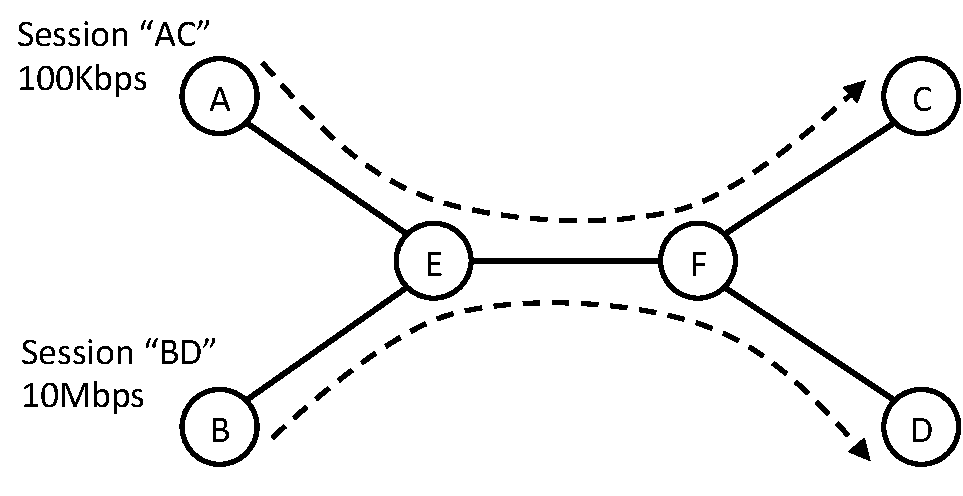
\includegraphics[scale=0.4] {figures/bottleneckExample.pdf}
\caption{Simple example of bottleneck inference algorithm.}
\label{fig:idea:example}
\end{center}
\end{figure}

\subsection{Bottleneck inference}
The basic idea of bottleneck inference algorithm is to rank the IP-level links along the routing path of each session by its likelihood to be the bottleneck link, called {\it Bottleneck Score}. Note that only using this technique, we cannot know for sure which link is the bottleneck link. Instead, this technique enables to identify the top 3 links that are most likely to be the bottleneck with higest Bottleneck Score. 

The algorithm is based on two assumptions:
\begin{packeditemize}
	\item {\bf A1:} The path available bandwidth is identical to available bandwidth of the bottleneck link, and 
	\item {\bf A2:} (Fairn share) All paths sharing the same bottleneck link should receive at most the available bandwidth on the link.
\end{packeditemize}
Consequently, we have the following statements: ``{\it Given two paths $P,P'$ such taht $P$ shares a link $L$ with $P'$, if $P'$ has a significantly higher bandwidth than $P$, then the bottleneck link of $P$ should not be $L$}''. The rationale is that otherwise, if $P$ is bottlenecked by link $L$, $P'$ should at most get $L$ ($A2$) which is identical to the bandwidth seen by $P$ ($A1$). However, this is contradict to the assumption. 
More realistically, taking into account other parameters (e.g., round trip time, slow start time), the bandwidth $P'$ sees could be a bit different from what $P$ sees. So we only consider ases where $P'$ has bandwidth much higher (e.g., more than 1Mbps higher) than $P$. For example, in Figure~\ref{fig:bottleneckExample}, since path from  $A$ to $C$ (100kbps) has significantly higher bandwidth than from $B$ to $D$ (10Mbps), their overlapping link between $E$ and $F$ should not be the bottleneck of path from A to C.

Based on this intuition, we calculate a Bottleneck Score for each link along a path that indicates how likely the link is to be a bottleneck as follows. Suppose that each path $P$ is a set of links along it, and for each link $L$ on path $P$, its Bottleneck Score is:

\begin{align*}
&BottleneckScore(L)\\
&=1-Pr\{BW(P') > 1.5\cdot BW(P) | L \in P \cap P'\}\\
&=1-\frac{|\{P'|\{BW(P') > 1.5\cdot BW(P), L \in P \cap P'\}|}{|\{P'|L \in P \cap P'\}|}
\end{align*}

Intuitively, the higher the Bottleneck Score is, the less other sessions indicating the link not being a bottleneck, and thus in other words, the more likely the link is the bottleneck. The technique will return the links with the highest score. 
One thing needs to note is that if a link is not shared with other path (i.e., $\{P'|L\in P\cap P'\}=\emptyset$), the Bottleneck Score will become meaningless. This is usually caused by last mile links that only connect to a few users.
To avoid this problem, we aggreage client and server IP into /24 blocks, and predict the bottleneck along the path between two IP blocks. 


To rule out possible bottleneck link by correlating paths is not first proposed -- \cite{} has mentioned the same idea and \cite{} used path comparison to find system bottleneck in other scenarios. However, our contribution lies in ...

\begin{figure}[h]
\begin{center}
%\includegraphics[]{p1_2Fig.ps}
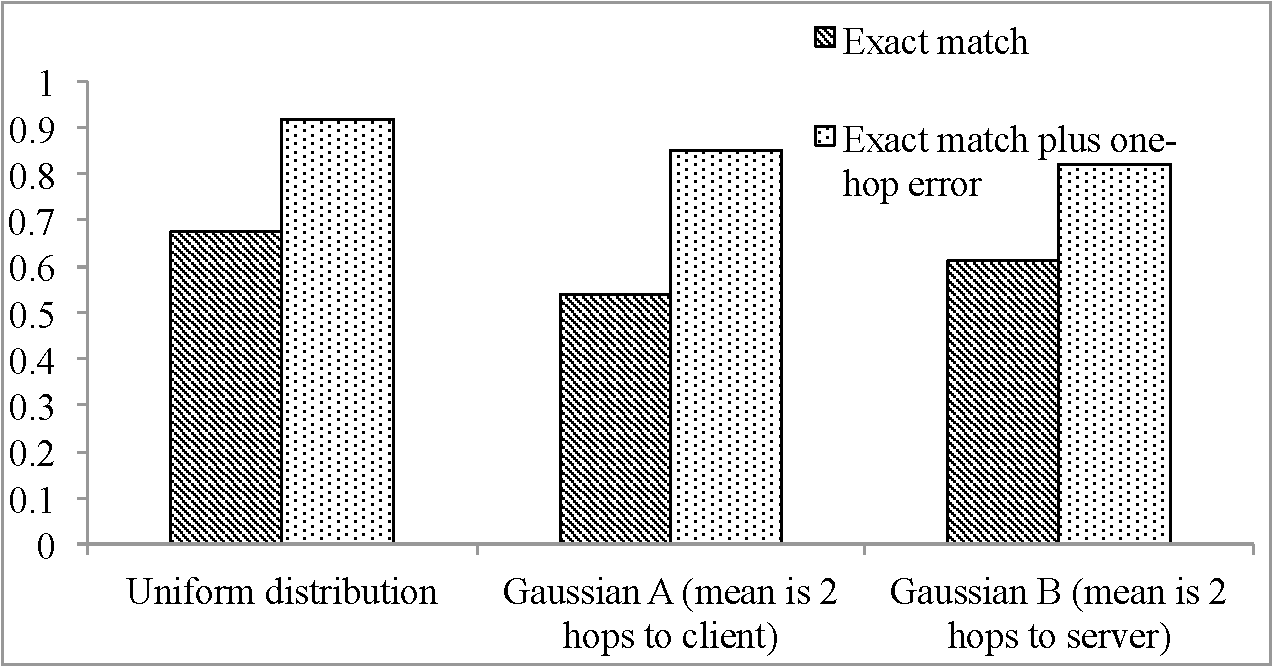
\includegraphics[scale=0.4] {figures/bottle-sim-bar.pdf}
\caption{Simulation-based validation for bottleneck inference technique under three bottleneck distributions. Y: the accuracy in identifying the bottleneck.}
\label{fig:cdn-criticalAttributeSets}
\end{center}
\end{figure}

\subsection{Data-driven simulation}
We now show a data-driven simulation to validate the proposed bottleneck inference technique and the validation results. The goal of the simulation is to test the feasibility of bottleneck inference technique -- if it can identify bottleneck links in a real topology, under various traffic pattern and bottleneck distribution. 

To this end, we use client requests in our own dataset and the path obtained from iPlane to generate a real network topology of links that have been probed by video sessions. We then randomly generate sessions between client and servers. In particular, we consider three bottleneck distributions -- uniformly distribution through the network, skewed distribution such that bottlenecks are close to clients, and skewed distribution such that bottlenecks are close to servers. To control the location of bottleneck for each session, we adjust the volume of background traffic on each link such that each session will be bottlenecked on a certain link (ground truth). Finally, we use only the available bandwidth of each session and run the bottleneck inference algorithm to localize the bottleneck links and compare it with the ground truth. Figure~\ref{fig:cdn-criticalAttributeSets} gives the result of bottleneck inference accuracy for three bottleneck distribution. Each of them has run for 30 times and we show the average value. The figure shows that for all three bottleneck distribution patterns, more than 80\% of the identified bottlenecks are no more than 1 hop from the real ones.. This error is tolerable in the hope that one hop will not significantly change the location of the bottleneck links.

